\documentclass[sigconf]{acmart}

\usepackage{booktabs} % For formal tables
\usepackage{hyperref}
\usepackage{amsmath}
\usepackage{amsthm}
%\usepackage{amsfonts}
%\usepackage{mathrsfs}
\usepackage[mathscr]{eucal}
%\usepackage{bm}
%\usepackage{bbm}
\usepackage{stmaryrd}
\usepackage{algorithm}
\usepackage{algorithmic}
\usepackage{footmisc}   % \footref, refer the same footnote at different places
%\usepackage{subcaption} % sub-figures
\usepackage{subfig} % sub-figures
\usepackage{setspace}   % set space between lines
\usepackage[utf8]{inputenc}
\usepackage[english]{babel}
\usepackage{xcolor}
\usepackage{graphicx}

\usepackage{enumerate}
\usepackage{accents}
\usepackage[framemethod=tikz]{mdframed}
\usepackage{colortbl}

\usepackage{tikz}
\usetikzlibrary{calc,fit,shapes,decorations.pathmorphing}

\graphicspath{{fig/}}   % Location of the graphics files

\DeclareMathOperator*{\argmin}{argmin}
\DeclareMathOperator*{\argmax}{argmax}
\newcommand{\eat}[1]{}
\newcommand{\given}{\mid}
\newcommand{\llb}{\llbracket}
\newcommand{\rrb}{\rrbracket}
\newcommand{\bu}{\mathbf{u}}
\newcommand{\bv}{\mathbf{v}}
\newcommand{\x}{\mathbf{x}}
\newcommand{\y}{\mathbf{y}}
\newcommand{\w}{\mathbf{w}}
\newcommand{\p}{\mathbb{P}}
\newcommand{\q}{\mathbf{q}}
\newcommand{\alphat}{\tilde{\alpha}}
\newcommand{\betat}{\tilde{\beta}}
\newcommand{\gammat}{\tilde{\gamma}}

\newcommand{\XCal}{\mathscr{X}}
\newcommand{\YCal}{\mathscr{Y}}
\newcommand{\PCal}{\mathscr{P}}

\newcommand{\OSf}{\mathsf{O}}
\newcommand{\SSf}{\mathsf{S}}
\newcommand{\defEq}{\stackrel{.}{=}}
%\newcommand{\argmax}{\operatorname{argmax}}

\newcommand{\indicator}[1]{\llbracket #1 \rrbracket}

\newcommand\thickbar[1]{\accentset{\rule{.4em}{.8pt}}{#1}}

\newcommand{\eg}{e.g.\ }
\newcommand{\ie}{i.e.\ }
\newcommand{\downto}{\,\textbf{downto}\,}
\newcommand{\blue}[1]{{\color{blue}{#1}}}


% Copyright
%\setcopyright{none}
%\setcopyright{acmcopyright}
%\setcopyright{acmlicensed}
\setcopyright{rightsretained}

% DOI
\acmDOI{10.475/123_4}

% ISBN
\acmISBN{123-4567-24-567/08/06}

% Conference
\acmConference[CitRec '17]{ACM RecSys Workshop on Recommender Systems for Citizens}{September 2017}{Como, Italy}
\acmYear{2017}
\copyrightyear{2017}
\acmPrice{15.00}

% Remove the non-mandatory "ACM Reference format."
%\fancyhead{}
%\settopmatter{printacmref=false, printfolios=false}

\allowdisplaybreaks

\begin{document}
\title{Revisiting revisits in trajectory recommendation}
%\titlenote{Produces the permission block, and copyright information}
%\subtitle{Extended Abstract}
%\subtitlenote{The full version of the author's guide is available as \texttt{acmart.pdf} document}

\author{Dawei Chen, Aditya Krishna Menon, Lexing Xie, Cheng Soon Ong}
\affiliation{%
 \institution{The Australian National University and Data61/CSIRO}
}
\email{ [u5708856, aditya.menon, lexing.xie, chengsoon.ong] @anu.edu.au}

\begin{abstract}
% !TEX root=./main.tex

%Playlists are a core feature of music streaming services.
Playlist recommendation concerns producing a sequence of songs that a user might enjoy.
We investigate this problem in three different cold-start scenarios:
%Specifically, we investigate three settings with different cold items:
(i) \emph{cold playlists}, where we recommend a set of songs to form a new playlist for an existing user; %without additional context except the user;
(ii) \emph{cold songs}, where we recommend newly released songs to extend existing playlists;
(iii) \emph{cold users}, where we recommend a set of songs to form a new playlist for a new user. %, without any other context.
%
We propose a flexible multitask learning method to deal with all three settings.
The method learns from user-curated playlists,
%the %multitask learning
%method
and encourages songs in the playlist 
to be ranked higher than those are not
by minimising a %the Bottom-Push
bipartite ranking loss.
We formulate the objective as a constrained convex optimisation problem,
and show how this may be approximated by an unconstrained objective
%then address the difficulty of a large number of constraints by approximating the %Bottom-Push loss
%bipartite ranking loss
%with a classification loss
inspired by an equivalence relationship between bipartite ranking and binary classification.
Empirical results on two real music playlist datasets show the proposed approach has good performance for playlist recommendation
in cold-start settings.
%in three cold-start settings.

\end{abstract}

%
% The code below should be generated by the tool at
% http://dl.acm.org/ccs.cfm
% Please copy and paste the code instead of the example below. 
%

%\keywords{ACM proceedings, \LaTeX, text tagging}

\maketitle

%%%%%%%%%
\section{Introduction}
% !TEX root=./main.tex

\section{Introduction}
\label{sec:intro}
Online music streaming services (e.g., Spotify, Pandora, Apple Music) % Google Play Music, Amazon Music) 
play an increasingly important role in the digital music industry.
A key ingredient of these services is the ability to automatically recommend songs to help users explore large collections of music.
%as well as create an uninterrupted listening experience.
Such recommendation is often in the form of a \emph{playlist}, 
%which is simply an ordered sequence of songs
which involves a (small) set of songs.
%
% one paragraph about recommender system
Conventional recommender systems for books or movies~\citep{Sarwar:2001,Netflix}
typically learn a score function via matrix factorisation~\citep{Koren:2009},
and recommend the item that achieves the highest score.
This approach is not suited to %deal with 
\emph{cold-start} settings,
where there is no historical data for either users or items.
%
% explain what is different about recommending playlist
Further, in playlist recommendation,
one has to recommend a subset of a large collection of songs instead of only one top ranked song.
Enumerating all possible such subsets is intractable;
additionally,
it is likely that more than one playlist is satisfactory, since
users generally maintain more than one playlist when using a music streaming service,
which leads to challenges in standard supervised learning.


%We investigate the problem of recommending a playlist of songs for a given user.
%If the user is new to the system, we would like to make a decent default recommendation by learning from 
%all available playlists of existing users.
%On the other hand, if the user already has a few playlists in the system, it is expected the recommender 
%system can also learn from this information and hopefully make better recommendations.
%
We investigate the problem of recommending songs to form personalised playlists %(for a given user)
in cold-start settings by learning from user-curated playlists.
%
%First, we study the problem of recommending a set of songs to form a playlist for a new user (\ie \emph{cold user}).
%We find it is challenging to improve recommendations beyond simply ranking songs according to their popularity,
%which is consistent with discoveries in~\cite{mcfee2012million,bonnin2013evaluating,bonnin2015automated}.
% the reason is believed to be that a small number of popular songs appeared in a large number of playlists, 
% and the majority of songs only appear in a few playlists~\cite{bonnin2013evaluating}.
% This is consistent with discoveries in~\cite{bonnin2013evaluating,jannach2015beyond,bonnin2015automated}
%
First, we study the problem of recommending a set of songs to form a new playlist for a user
%We learn the preference of the given user from her existing playlists,
by exploiting the (implicit) preference %of the given user 
from her existing playlists.
We find that learning from a user's existing playlists %can significantly 
improves the accuracy of recommendation.
Since we do not have any contextual information about the new playlist, 
we call this setting \emph{cold playlists}.
%
We further consider the setting of new users (\ie \emph{cold users}),
where we recommend playlists for new users.
We find it challenging to improve recommendations beyond simply ranking songs according to their popularity 
if we know nothing about the user, which is consistent with previous 
discoveries~\cite{mcfee2012million,bonnin2013evaluating,bonnin2015automated}.
However, improvement can still be achieved if we know a few simple attributes (\eg age, gender, country etc.)
of the users.
%
%This motivates us to exploit the (implicit) user preference from her existing playlists,
%which leads to the \emph{cold playlists} setting,
%where a set of songs are recommended to form a new playlist for an existing user. %of a music service.
%We find that learning from a user's existing playlists %can significantly 
%improves the accuracy of recommendation.
%
%In addition, 
%We further investigate the value of seed songs for improving recommendation.
%This results in the \emph{cold songs} setting,
%where we recommend a set of newly released songs to extend users' existing playlists. %from users.
%
Lastly, we investigate the problem of recommending newly released songs (\ie \emph{cold songs}) to extend users' existing playlists. 
We find that songs in a playlist are especially helpful in guiding the process of adding new songs to a given playlist.
%We call this setting \emph{cold songs}.



% The challenge of this task, besides those brought by cold-start settings, is two-fold:
% \begin{enumerate}[(i)]
%	\item \emph{Sparsity}. While a large number of playlists are hosted by music streaming services,
% playlists for each user is still limited. This is exacerbated by the long-tailed distribution that
% most users only have a few playlists, while a small portion of users have a very large number of playlists.
% Similarly, a small number of popular songs appeared in a large number of playlists, and the majority of songs
% only appear in a few playlists~\cite{bonnin2013evaluating}.
%	\item \emph{Noise}. There could be noise in metadata~\cite{bonnin2015automated} or users might randomly choose songs 
% from their music collection when composing playlists~\cite{mcfee2012hypergraph}.
%% which makes it hard to learn the intent of a playlist.
% \end{enumerate}
%These challenges make it hard to make recommendations better than simply ranking songs according to their 
% popularity~\cite{mcfee2012million,bonnin2013evaluating,bonnin2015automated},



%%In this paper, we propose a novel approach which ranks 
% In this paper, we propose a novel multitask learning method for playlist recommendation in cold-start settings.
We propose a novel multitask learning method that %to %which can 
%deals with 
can handle
all three cold-start settings for playlist recommendation.
%It aims to 
It learns to rank songs that are likely to be in a playlist %that could end up being in a playlist %for the given user 
above those unlikely to be chosen. %by minimising a bipartite ranking loss.
%
%To learn the parameters, 
We optimise the multitask learning objective by formulating %solving 
%which involves 
a constrained convex optimisation problem.
To avoid dealing with an enormous number of constraints,
we approximate an optimal solution %of the multitask learning objective
by minimising an unconstrained objective 
inspired by an equivalence %relationship 
between bipartite ranking and binary classification.
%
%we approximate an optimal solution of the multitask learning objective by minimising an unconstrained classification loss.
%we show how one can approximate the multitask objective to avoid dealing with a large number of constraints.
%using an equivalence relationship between bipartite ranking and binary classification.
%This results in an unconstrained objective that approximates the multitask objective.
%
We present experiments on two real playlist datasets, %for all three cold-start settings,
and demonstrate that our multitask learning approach improves over existing strong baselines 
for playlist recommendation in cold-start scenarios.
%
%This approach achieves good performance in cold-start playlist recommendation on two real playlist datasets.
%
%Experiments on two real playlist datasets show the proposed approach 
%has good performance for playlist recommendation in cold-start scenarios. %settings.
%and the classification approach in particular significantly improves the learning efficiency 
%while maintaining the same level of high performance as the ranking approach.
%
% Our paper is organised as follows:
% Section 2 discusses previous study that are most relevant to our work.
%%Section 2 illustrates the three cold-start settings we investigate and summarises recent related work.
%Section 3 describes the multitask objective and approaches to optimise it.
%%a bipartite ranking loss which aims to ranks songs in a playlist higher than those are not.
%%We optimises the multitask objective by solving a constrained optimisation problem.
%%We then describe a classification loss which enables us to approximately optimise the objective by
%%solving an unconstrained optimisation problem.
%%Section 4 discusses previous work that are most relevant to our work.
% Section 4 details experiments of cold-start playlist recommendation. % on two real playlist datasets.
% Lastly, we summarises the paper and describes future work in Section 5.


%\setlength{\belowdisplayskip}{1pt} \setlength{\belowdisplayshortskip}{0pt}
%\setlength{\abovedisplayskip}{1pt} \setlength{\abovedisplayshortskip}{0pt}

%%%%%%%%%
\section{Trajectory \& path recommendation}
\label{sec:background}
% !TEX root=main.tex

We now formalise the problem of interest and outline its challenges.

%
\subsection{Trajectory recommendation}

Fix some set $\PCal$ of points-of-interest (POIs) in a city.
A \emph{trajectory}\footnote{In graph theory, this is also referred to as a walk.} is any sequence of POIs, possibly containing loops (repeated POIs).
In the \emph{trajectory recommendation} problem, we are given as input a training set of historical tourists' trajectories.
From this, we wish to design a \emph{trajectory recommender}, which accepts a
\emph{trajectory query} $\x = (s, l)$, comprising a start POI $s \in \PCal$, and trip length $l \!>\! 1$, %(\ie the desired number of POIs, including $s$),
and produces one or more sequences of $l$ POIs starting from $s$. %that conform to the query.

Formally, let $\XCal \defEq \PCal \times \{ 2, 3, \ldots \}$ be the set of possible queries,
$\YCal \defEq \bigcup_{l = 2}^\infty \PCal^l$ be the set of all possible trajectories,
and for fixed $\x \in \XCal$, $\YCal_{\x} \subset \YCal$ be the set of trajectories that conform to the constraints imposed by $\x$,
\ie if $\x = (s, l)$ then $\YCal_{\x} = \PCal^l$.
Then, the {trajectory recommendation} problem has:

\vspace{0.5\baselineskip}

\begin{mdframed}[innertopmargin=3pt,innerbottommargin=3pt,skipbelow=5pt,roundcorner=8pt,backgroundcolor=red!3,topline=false,rightline=false,leftline=false,bottomline=false]
	\begin{tabular}{ll}
		{\sc Input}:  & training set $\left\{ \left( \x^{(i)}, \y^{(i)} \right) \right\}_{i = 1}^n \in ( \XCal \times \YCal )^n$ \\
		{\sc Output}: & a trajectory recommender $r \colon \XCal \to \YCal$ \\
	\end{tabular}
\end{mdframed}

\vspace{0.5\baselineskip}

One way to design a trajectory recommender is to find a (query, trajectory) affinity function $f \colon \XCal \times \YCal \to \mathbb{R}$, and let
\begin{equation}
	\label{eqn:argmax}
	r( x ) \defEq \argmax_{\y \in \YCal_x}~f(\x, \y).
\end{equation}
%In particular, $\y = (s,~ y_2, \dots, y_l)$ is a trajectory with $l$ POIs. %, which has no sub-tours. %i.e. $y_j \ne y_k$ if $j \ne k$.
%This was the view proposed in~\cite{cikm16paper} where they authors considered an
%objective function that added two components together: a POI score and a transition score.
Several choices of $f$ are possible.
\citet{cikm16paper} proposed to use $f$ given by a RankSVM model. %, combined with a transition score between POIs.
While offering strong performance, this has a conceptual disadvantage highlighted in the previous section:
it does not model global cohesion, and could result in solutions such as recommending three restaurants in a row.

To overcome this, \citet{Chen:2017} proposed to use $f$ given by a structured SVM (SSVM),
wherein $f( \x, \y ) = \mathbf{w}^T \Phi( \x, \y )$ for a suitable feature mapping $\Phi$.
%In the case of an SSVM with pairwise potentials,
When this feature mapping decomposes into terms that depend only on adjacent elements in the sequence $\y$ (akin to a linear-chain conditional random field),
the optimisation in Equation \ref{eqn:argmax} can be solved with the classic Viterbi algorithm.

% !TEX root=main.tex

\tikzstyle{state}=[shape=circle,draw=blue!50,fill=blue!20]
\tikzstyle{state2}=[shape=circle,draw=purple!50,fill=purple!20]
\tikzstyle{hiddenState}=[shape=circle,draw=gray!50,fill=gray!20,dashed]
\tikzstyle{specialState}=[shape=circle,double=red,draw=blue!50,fill=blue!20,dashed]
\tikzstyle{observation}=[shape=rectangle,draw=orange!50,fill=orange!20]
\tikzstyle{hiddenObservation}=[shape=rectangle,draw=gray!50,fill=gray!20,dashed]
\tikzstyle{lightedge}=[<-,thin]
\tikzstyle{mainstate}=[state,ultra thick]
\tikzstyle{mainedge}=[<-,ultra thick]

\begin{figure*}[!htb]
    \centering
    %\resizebox{0.2\textwidth}{!}{
    \subfloat[{\sc LoopElim} (\S\ref{sec:loop-elim}).]{
    \begin{tikzpicture}[baseline=(s0.base)]
        % states
        \node[specialState] (s0) at (0,0) {$1$};
        \node[specialState] (s1) at (1,0) {$2$}
            edge [<-,ultra thick] (s0);
        \node[specialState] (s2) at (2,0) {$3$}
            edge [<-,ultra thick] (s1);
        %\node[state] (s3) at (3,0) {$4$}
        %    edge [<-,ultra thick] (s2);
        
        %\draw [<-,ultra thin,bend right] (s1) to [looseness=1.25] (s3) node[sloped,draw=none] at (2,-0.45) {$/$};
        \draw [<-,ultra thin,bend right] (s0) to [looseness=1.25] (s2) node[sloped,draw=none] at (1,-0.45) {$/$};

        \node[draw=none] at (0,-1.15)  {};
    \end{tikzpicture}
    %}
    }%
    \qquad    
    %\subfloat[Original prediction with loop (dashed).]{
    \subfloat[{\sc Greedy} (\S\ref{sec:greedy}).]{
    \begin{tikzpicture}[baseline=(s12.base)]
        % first-best
        \node[specialState] (s11) at (0,1)  {$1$};
        \node[hiddenState]  (s12) at (0,0)  {$2$};
        \node[hiddenState]  (s13) at (0,-1) {$3$};

        %\node[hiddenState] (s2) at (1,1.5)  {$2$};
        \node[hiddenState]  (s21) at (1,1)  {$1$};
        \node[specialState] (s22) at (1,0)  {$2$};
        \node[hiddenState]  (s23) at (1,-1) {$3$};
        %\node[hiddenState] (s6) at (1,-1.5)  {$6$};

        \node[draw=none] (s32) at (2,1)  {};
        \node[draw=none] (s31) at (2,0)  {};
        \node[draw=none] (s33) at (2,-1) {};

        \node[draw=none] (s411) at (2.25,0)     {$\ldots$};

        %\draw [->,ultra thin] (s1) to (s2);
        \draw [->,ultra thin]      (s11) to (s21) node [draw=none] at (0.5,1) {$/$};
        \draw [->,ultra thick] (s11) to (s22);
        \draw [->,ultra thin]  (s11) to (s23);
        %\draw [->,ultra thin] (s1) to (s6);

        \draw [->,ultra thin] (s22) to (s32) node [draw=none] at (1.5,0.5) {$/$};
        \draw [->,ultra thin] (s22) to (s31) node [draw=none] at (1.5,0)     {$/$};
        \draw [->,ultra thin] (s22) to (s33);
    \end{tikzpicture}
    }%   
    \qquad
    % \subfloat[Modified prediction with loop removed.]{
    % \begin{tikzpicture}[baseline=(s0.base)]
    %     % states
    %     \node[state] (s0) at (-2,2) {$1$};
    %     \node[state] (s1) at (0,2) {$2$}
    %         edge [<-] (s0);
    %     \node[state] (s2) at (2,2) {$3$}
    %         edge [<-] (s1);
    %     \node[state] (s3) at (4,2) {$4$}
    %         edge [<-] (s2);
    %     \draw [color=white,dashed,bend right] (s1) to [looseness=1.25] (s3);            
    % \end{tikzpicture}
    % }
    %\resizebox{0.2\textwidth}{!}{
    \subfloat[{\sc ILP} (\S\ref{sec:ilp}).]{
    \begin{tikzpicture}[baseline=(s1.base)]
        % first-best
        \node[specialState] (s1) at (0,0)  {$1$};
        \node[specialState] (s2) at (1,1)  {$2$};
        \node[hiddenState]  (s3) at (2,1)  {$3$};
        \node[hiddenState]  (s4) at (1,-1) {$4$};
        \node[specialState] (s5) at (2,-1) {$5$};
        \node[specialState] (s6) at (3,0)  {$6$};

        %\node[draw=none] (juka) at (0,-1.5)  {};

        \draw [->,ultra thick] (s1) to (s2);
        \draw [->,ultra thin] (s1) to (s3);
        \draw [->,ultra thin] (s1) to (s4);
        \draw [->,ultra thin] (s1) to (s5);
        \draw [->,ultra thin] (s1) to (s6);    

        \draw [->,ultra thin] (s2) to (s1);
        \draw [->,ultra thin] (s2) to (s3);
        \draw [->,ultra thin] (s2) to (s4);
        \draw [->,ultra thick] (s2) to (s5);
        \draw [->,ultra thin] (s2) to (s6);    

        \draw [->,ultra thin] (s3) to (s1);
        \draw [->,ultra thin] (s3) to (s2);
        \draw [->,ultra thin] (s3) to (s4);
        \draw [->,ultra thin] (s3) to (s5);
        \draw [->,ultra thin] (s3) to (s6);    

        \draw [->,ultra thin] (s4) to (s2);
        \draw [->,ultra thin] (s4) to (s3);
        \draw [->,ultra thin] (s4) to (s1);
        \draw [->,ultra thin] (s4) to (s5);
        \draw [->,ultra thin] (s4) to (s6);    

        \draw [->,ultra thin] (s5) to (s2);
        \draw [->,ultra thin] (s5) to (s3);
        \draw [->,ultra thin] (s5) to (s4);
        \draw [->,ultra thin] (s5) to (s1);
        \draw [->,ultra thick] (s5) to (s6);    

        \draw [->,ultra thin] (s6) to (s2);
        \draw [->,ultra thin] (s6) to (s3);
        \draw [->,ultra thin] (s6) to (s4);
        \draw [->,ultra thin] (s6) to (s5);
        \draw [->,ultra thin] (s6) to (s1);                    
    \end{tikzpicture}
    %}
    }%
    \qquad
    \subfloat[{\sc List Viterbi} (\S\ref{sec:viterbi}).]{
    \begin{tikzpicture}[baseline=(s1.base)]
        % first-best
        \node[specialState] (s1) at (0,0)  {$1$};
        \node[specialState] (s2) at (1,0)  {$2$}            
            edge [<-,ultra thick] (s1);

        \node[specialState] (ss1) at (2,-1) {{${5}$}}
        	edge [<-,ultra thick,decorate,decoration={snake}] (s2);
        \node[specialState] (ss2) at (3,-1) {{${6}$}}
            edge [<-,ultra thick,decorate,decoration={snake}] (ss1);

        \node[hiddenState] (s3) at (2,0)  {$3$}            
            edge [<-,ultra thin] (s2);

        % \node[hiddenState] (s4) at (3,0) {$4$}
        %     edge [<-,ultra thin] (s3);

        %\draw [<-,ultra thin,bend left] (s2) to [looseness=1.25] (s4); 
        \draw [<-,ultra thin,bend left] (s1) to [looseness=1.25] (s3); 
    \end{tikzpicture}
    }
    
    %\caption{Example of heuristically removing loops. The nodes are numbered by the POI, with edges denoting order in the sequence. While the modified prediction removes the loop in the original sequence, it is necessarily at the expense of returning a path with fewer number of POIs.}
    \caption{Schematics of different algorithms to return a loop-free prediction.
    Nodes such as
	{\protect\tikz[baseline=(X.base)]{\protect\node[specialState,inner sep=2pt] (X) {\small$1$}}}
    are selected by the algorithm, with thick edges such as
    {\protect\tikz{\protect\coordinate (X) at (0,0) {}; \protect\coordinate (Y) at (0.5,0) {}; \protect\draw[->,ultra thick] (X) to (Y); \protect\node[draw=none] at (0.25,-0.00625) {}}}
    denoting the sequence ordering.
    {\sc LoopElim} removes the loop from the Viterbi solution (here the POI sequence $(1,2,3,1)$), possibly returning a path of shorter length than requested;    
    {\sc Greedy} incrementally selects POIs which locally maximise the sub-path score, and have not been selected before;
    {\sc ILP} solves an integer linear program to find the optimal length $l$ path in a complete graph over POIs;
    {\sc ListViterbi} finds where the second-best sequence diverges from the standard Viterbi sequence ($(1,2,3,1)$ as before); if not loop-free, it finds where the third-best diverges from the second-best, \emph{etc}.
    }
    \label{fig:schematics}
    \vspace{-0.5\baselineskip}
\end{figure*}



%
\subsection{Path recommendation}

We argue that the definition of trajectory recommendation is incomplete for a simple reason:
in most cases, a tourist will not want to revisit the same POI.
Instead, what is needed is to recommend a \emph{path}, \ie a trajectory that does not have any repeated POIs.
Let $\thickbar{\YCal} \subset \YCal$ be the set of all possible paths,
and for fixed $\x \in \XCal$, let $\thickbar{\YCal}_{\x} \subset \thickbar{\YCal}$ be the set of paths that conform to the constraints imposed by $\x$.
We now wish to construct a \emph{path recommender} $r \colon \XCal \to \thickbar{\YCal}$ via
\begin{equation}
	\label{eqn:argmax-path}
	r( x ) \defEq \argmax_{\y \in \thickbar{\YCal}_x}~f(\x, \y).
\end{equation}
For $f$ given by an SSVM, Equation \ref{eqn:argmax-path} requires we depart from the standard Viterbi algorithm, as the sequence in Equation \ref{eqn:argmax} may well have a loop.\footnote{In SSVMs, this issue also arises during training \citep{Chen:2017}, but we focus here only on the prediction problem. See \S\ref{sec:discussion} for additional comments.}
There are two distinct modes of attack available:
\begin{enumerate}
	\item seek an approximate solution to the problem,
	via heuristics that exploit a graph view of Equation \ref{eqn:argmax-path}.
	%that remove loops present in the standard Viterbi solution,
	%or by greedily constructing a loop-free solution.

	\item seek an exact solution to the problem,
	via integer linear programming,
	or top-$K$ extensions of the Viterbi algorithm. %(known as list Viterbi algorithms).
\end{enumerate}
While \citet{Chen:2017} suggested the latter exact approaches, they did not formally compare their performance either qualitatively or quantitatively;
they did not detail the different top-$K$ extensions of the Viterbi algorithm and the connections thereof;
and they did not consider approximate approaches.

In the sequel, we thus detail the above approaches in more detail.
Figure \ref{fig:schematics} gives a schematic overview of these algorithms.


% {\color{red!75}
% \begin{itemize}
%   %\item connect to workshop
%   %\item distinguish between next location vs whole trajectory
%   %\item define word usage: trajectory, path, walk, sequence, tour, etc.
%   \item describe relation to travelling salesman, and say why different
%   %\item contributions of this paper
% \end{itemize}
% }


%%%%%%%%%
\section{Graph-based heuristics}
\label{sec:heuristics}
% !TEX root=main.tex

To design approximations, it will be useful to view Equation \ref{eqn:argmax-path} as a graph optimisation problem
for the case of structured SVMs with pairwise potentials.
Here, the score $f(\mathbf{x}, \mathbf{y})$ can be decomposed as
%$$ f(\mathbf{x}, \mathbf{y}) = \sum_{k = 1}^{|\mathbf{y}|} \mathbf{w}_k^T \Phi( \mathbf{x}, y_k ) + \sum_{j, k = 1}^{|\mathbf{y}|} \mathbf{w}_{j k}^T \Phi( \mathbf{x}, y_k, y_j ) $$
%for unary and pairwise weight vectors $\mathbf{w}_k$.
\begin{equation}
	\label{eqn:f-ssvm}
	f(\mathbf{x}, \mathbf{y}) = \sum_{k = 1}^{|\mathbf{y}|} \alpha( y_k ) + \sum_{k = 1}^{|\mathbf{y}| - 1} \beta( y_k, y_{k+1} )
\end{equation}
for suitable unary and pairwise potentials $\alpha, \beta$.
Consequently, we can imagine a complete graph where the nodes are POIs, each node $p \in \PCal$ has a score $\alpha( p )$, and each edge $(p, p') \in \PCal^2$ has a score $\beta( p, p' )$.
Then, Equation \ref{eqn:argmax-path} is equivalently a problem of selecting $l$ nodes such that
the total sum of node and edge scores in the selection maximises Equation \ref{eqn:f-ssvm}.
% This points to a natural means of approximation: solve this selection problem greedily, or fix the set of nodes and only solve the ordering problem.
%the following selection problem:
%$$	r( x ) = \argmax_{\mathbf{y} \in \thickbar{\YCal}_x}~\sum_{k = 1}^{|\mathbf{y}|} \alpha( y_k ) + \sum_{j, k = 1}^{|\mathbf{y}|} \beta( y_k, y_j ). $$
We now look at ways of approximately solving this selection problem.

\subsection{Greedy path discovery}
\label{sec:greedy}
% !TEX root=main.tex

In light of the graph-based view, a natural approach to approximately solve Equation \ref{eqn:argmax-path} is a greedy algorithm.
Suppose we have already determined a partial path comprising distinct POIs $y_1, \ldots, y_k$.
Then, we can select the next candidate POI $y_{k + 1}$ as
the node
that iteratively optimises Equation \ref{eqn:f-ssvm},
%whose combined node- and edge-score is maximum,
subject to the constraint that it is distinct from all other nodes in the current path;
formally, we pick
%the node whose combined node score $\alpha( y_{k + 1} )$ and
%transition score $\beta( y_{k}, y_{k + 1} )$
$$ y_{k + 1} = \argmax_{p \in \PCal - \{ y_1, \ldots, y_k \}} \alpha( p ) + \beta( y_k, p ). $$
This algorithm is faster that the above heuristic, with $\mathscr{O}(l \cdot | \PCal |)$ complexity,
but similarly has an unclear performance guarantee.


\subsection{Heuristic loop elimination}
\label{sec:loop-elim}
% !TEX root=main.tex

An even simpler approach than the above greedy strategy is the following:
by default, return the standard Viterbi solution (Equation \ref{eqn:argmax});
if this solution has loops, then simply remove them.
Specifically, if the Viterbi solution is $( y_1, \ldots, y_l )$,
and $i$ is the first index where $y_i$ already appears in the subsequence $( y_1, \ldots, y_{i-1} )$,
then simply return the subsequence $( y_1, \ldots, y_{i-1} )$.

The above algorithm is guaranteed to return a path,
but has at least two detrimental features.
First, it returns a solution that violates the length constraint of the trajectory recommendation problem.
Second, if we restrict attention to the POIs $\{ y_1, \ldots, y_{i-1} \}$, it is unclear whether the original ordering of the subsequence is optimal.
The second point can be remedied, as we now see.


% \subsection{Heuristic subtour elimination}
% \label{sec:christofides}
% % !TEX root=main.tex

%\blue{How to use results from travelling salesman for trajectory recommendation?} 

%\noindent
The problem of recommending a trip over a set of POIs can be reduced to the classic travelling salesman problem (TSP)
if every POI is restricted to visit once.
However, in practice, we normally only visit a subset of these POIs,
which means results of TSP cannot be trivially used unless the subset of POIs is fixed.

%\noindent
%\blue{Not obvious how to directly use Christofides? Do we just find double visits and bypass?} 
%https://research.googleblog.com/2016/09/the-280-year-old-algorithm-inside.html

%\noindent
One well-known heuristic to approximately solve the TSP is the Christofides algorithm \citep{Christofides:1976}.
This algorithm finds a circuit that cost at most 1.5 times
of the optimal TSP solution, by constructing a minimum spanning tree and matching certain nodes, 
building the solution by simply bypassing repeated nodes.

Inspired by this, and recalling that the recommended trips by the classic Viterbi algorithm cannot avoid repeated visits,
we can first request a longer sequence using Viterbi and then skip repeated visits to form a trip, 
we keep asking for sequence with different length, until we cannot improve the resulting trip (with respect to the required length).
This algorithm is denoted as \textsc{Heuristic} in experiment.



%%%%%%%%%
%\section{Subtour Elimination using Integer Programming}
%\section{Subtour Elimination using ILP}
\section{Integer Linear Programming \& TSP}
\label{sec:ilp}
% !TEX root=main.tex

We should probably ask Phil Kilby or Hassan about the two or three most popular subtour eliminations

\begin{itemize}
	\item Elementary shortest path problems
  %http://www.optimization-online.org/DB_FILE/2014/09/4560.pdf
	\item Different subtour eliminations
  	\item (Dantzig, Fulkerson, Johnson, 1954) has 3 different versions
  	\item (Miller, Tucker, Zemlin, 1960) has another one.
  	\item Seems to be one more, not sure by whom (maybe Belmore, Malone, 1971)
  %http://www.or.unc.edu/~pataki/papers/teachtsp.pdf

\end{itemize}


%%%%%%%%%
\section{Top-k Sequences using List Viterbi}
\label{sec:viterbi}
% !TEX root=main.tex

% \begin{itemize}
%     %\item use list viterbi to go down top-k best sequences until we find one without loops
%     %\item two versions of serial list viterbi are equivalent
%     %\item parallel list viterbi
% \end{itemize}

The Viterbi algorithm %for standard inference in a structured prediction model.
%This
finds the best scoring sequence in Equation \ref{eqn:argmax}, which may have loops.
To find the best sequence without loops in Equation \ref{eqn:argmax-path}, one can apply a \emph{list Viterbi algorithm}
to find not just the single best sequence,
but rather the top $K$ best sequences.
By definition, the first such sequence that is loop free must be the highest scoring sequence that does not have loops.
We detail existing approaches to solving the list Viterbi problem.

%
\subsection{Parallel and serial list Viterbi algorithms}

At a high level, there are two approaches to extend the Viterbi algorithm to the top-$K$ setting.
The first approach is to keep track, at each state, of the top $K$ sub-sequences that end at this state; these are known as \emph{parallel list Viterbi} algorithms.
Such algorithms date back to at least \citet{Forney:1973},
but have the disadvantage of imposing a non-trivial memory burden.
Further, they are not applicable as-is in our setting:
we do \emph{not} know in advance what value of $K$ is suitable,
since we do not know the position of the best loop-free sequence.

The second approach is to more fundamentally modify how one selects paths; these are known as \emph{serial list Viterbi} algorithms.
Amongst serial list Viterbi algorithms, there are at least two well-known proposals in the context of hidden Markov models (HMMs).
In the signal processing community, \citet{seshadri1994list} proposed an algorithm that keeps track of the ``next best'' sequence terminating at each state in the current list of best sequences.
In the AI community, \citet{nilsson2001sequentially}
%(building on the work of \citet{Nilsson:1998} for general graphical models)
proposed an algorithm that cleverly partitions the search space into subsets of sequences that share a prefix with the current list of best sequences.
While derived in different communities, these two algorithms are in fact only superficially different, as we now see.

%
\subsection{Relating serial list Viterbi algorithms}

The connection between the existing list Viterbi algorithms is easiest to see in the case of finding the second best sequence for an HMM.
Suppose we have an HMM with states $\SSf_{t}$, observations $\OSf_{t}$, transition probabilities $a_{ij} = \Pr( \SSf_{t+1} = j \mid \SSf_t = i )$, and emission probabilities $b_{ik} = \Pr( \OSf_{t} = k \mid \SSf_t = i )$.
Suppose $s^*_{1:T}$ is the most likely length $T$ sequence given observations $\OSf_{1:T}$,
$\delta_{j, t}$ is the value of the best sequence up till position $t$ ending at state $j$ as computed by the Viterbi algorithm,
%$\delta_{j, t} \defEq \max_{\SSf_{1:t - 1}} \Pr( \SSf_{1:t - 1}, \SSf_t = j, \OSf_{1:t} )$
and our interest is in finding the second best sequence given observations $\OSf_{1:T}$, with value
$ M \defEq \max_{\SSf_{1:T} \neq s^*_{1 : T}}{\Pr( \SSf_{1:T}, \OSf_{1:T} )}. $

\citet{seshadri1994list} proposed to find $M$ via a recurrence similar to the standard Viterbi algorithm,
\begin{equation}
    \label{eqn:att-recurrence}
    \begin{aligned}
        M &= \bar{\delta}_{T+1} \\
        %(\forall t > 0) \,
        \bar{\delta}_t &= 
        \indicator{t > 0} \cdot
        \max
        \begin{cases}
        \max_{i \neq s^*_{t-1}} \delta(i, t-1) \cdot a( i, s^*_{t} ) \cdot b( s^*_{t}, \OSf_{t} ) \\
        \bar{\delta}_{t - 1} \cdot a( s^*_{t - 1}, s^*_{t} ) \cdot b( s^*_{t}, \OSf_{t} ).
        \end{cases}% \\
        %\bar{\delta}_0 &= 0.
    \end{aligned}    
\end{equation}
Intuitively, $\bar{\delta}_t$ finds the value of the second best sequence that merges with the best sequence by at least time $t$.
On the other hand, \citet{nilsson2001sequentially} proposed to find $M$ more directly via
\begin{align*}
	M &= \max_t \widehat{\rho}_t \\
	\widehat{\rho}_{t} &\defEq \max_{i \neq s^*_{t}} \max_{S_{t+1:T}} {\Pr( \SSf_{1:t-1} = s^*_{1:t-1}, \SSf_t = i, \SSf_{t+1:T}, \OSf_{1:T} )}.
\end{align*}
Intuitively, $\widehat{\rho}_t$ finds the value of the second best sequence that first deviates from the best sequence exactly at time $t$.
\citet{nilsson2001sequentially} propose to compute $\widehat{\rho}_{t}$ via the forward-backward values $\eta_{i, j, t} \defEq \max_{\SSf \colon S_{t - 1} = i, \SSf_{t} = j} \Pr( \SSf_{1:T}, \OSf_{1:T} )$,
which in turn can be computed from the ``backward'' analogue of $\delta$.

To connect the two approaches, observe that by unrolling the recurrence in Equation \ref{eqn:att-recurrence}, and definition of $\delta$, we have
\begin{align*}
	M &= \max_t \widehat{\mu}_t \\
	\widehat{\mu}_{t} &\defEq \prod_{k = 1}^t a( s^*_{k-1}, s^*_{k} ) \cdot b( s^*_{k}, \OSf_{k} ) \cdot \max_{i \neq s^*_{t}} \delta(i, t) \cdot a( i, s^*_{t+1} ) \cdot b( s^*_{t+1}, \OSf_{t+1} ) \\
	&= \max_{i \neq s^*_{t}} \max_{S_{1:t-1}} {\Pr( \SSf_{1:t}, \SSf_t = i, \SSf_{t+1:T} = s^*_{t+1:T}, \OSf_{1:T} )};
\end{align*}
i.e., the same quantities are computed, except that the former fixes the suffix of the candidate sequence, while the latter fixes the prefix.


%\section{List Viterbi algorithm}
\label{sec:lva}

There are many variants of generalising the Viterbi algorithm (VA) to find the 
$1$st, $2$nd, $\dots$, $k$-th best sequences~\cite{seshadri1994list,nilsson2001sequentially},
here we call them the list Viterbi algorithm (LVA).

We compare three typical variants of the LVA, mainly their time/space complexity.
Firstly, we define notations that will be used in this section, we denote:
\begin{itemize}
\item $n$: the (maximum) number of states of (all) random variables in the HMM.
\item $l$: the length of sequence, \ie, the number of random variables in the chain.
\item $k$: the total number of best sequences that are going to be identified.
\end{itemize}
We will also use $i$ to index the possible states of random variables, \ie, $i \in \{1, \dots, n\}$,
and use $t$ to index the locations/(time instants) in the chain/sequence, \ie, $t \in \{1, \dots, l\}$.

\subsection{Parallel LVA}
\label{sec:plva}

The parallel LVA finds the $k$ best sequences simultaneously by computing the $k$ best sequences in each state at each time instant.
The basic idea of parallel LVA is storing all the $k$ best scores instead of the $1$st best score in VA at each time instant,
which means we need to find the $k$ best scores among the $n\cdot k$ accumulated scores at each state and time instant 
(Eq. (6) in~\cite{seshadri1994list}).

The time complexity for this step (Eq. (6) in~\cite{seshadri1994list})
is $O \left( nk\cdot \log(nk) \right)$ if the $k$ best scores are found by sorting the $n\cdot k$ accumulated scores,
or $O \left( k \cdot nk \right)$ if the $k$ best scores are found by order statistics algorithms~\cite{clrs2009}, 
which is more expensive if $k$ is very large (\ie when $k > \log(nk)$),
so for this analysis, we assume this step is implemented by sorting.
As we are doing this step at each state and time instant, the total time complexity is $O \left( n \cdot l \cdot nk \cdot \log(nk) \right)$.
Intuitively, we are computing elements in a cube $n \times l \times k$, 
the third dimension needs a sorting to get the $k$ best elements in $nk$ elements.

The space complexity is $O ( nlk + nk )$, \ie $O(nlk)$ for all sequence states and $O(nk)$ for $nk$ accumulated scores at each time instant.


\subsection{Serial LVA}
\label{sec:slva}

In practice, we usually do not know the value of $k$ beforehand, this is where the serial LVA comes into play.
The serial LVA finds the $k$ best sequences one at a time, which is more flexible than the parallel LVA described in Section~\ref{sec:plva}.
This algorithm makes use of the observation that the globally $2$nd best sequence diverges from the globally $1$st best sequence 
at some time instant, and it merges with the globally $1$ best sequence at a later time instant and never diverges again, 
since any subsequent divergence will result in a higher cost (lower priority) sequence.
Similarly, the $3$rd globally best sequence can be identified from the locally $2$nd best sequences w.r.t. the globally $1$ best sequence 
(except the globally $2$ best sequence) or the locally $2$nd best sequences w.r.t. the globally $2$nd best sequence.
This reasoning can be generalised to find the $k$-th best sequence given the $1$st, $2$nd, \dots, $(k-1)$-th best sequences.

The time complexity of the serial LVA is composed of three parts:
\begin{itemize}
\item using the Viterbi algorithm to find the globally best sequence: $O(n^2 l)$ as the $n$-by-$l$ table stores scores and 
      computing each cell is upper bounded by $O(n)$.
\item computing locally $2$nd best sequences after identifying the globally $j$-th $(j=1,\dots,k-1)$ best sequence, 
      which requires $n$ additions and comparisons (Eq. (9) in~\cite{seshadri1994list}) at each time instant $t \in \{1, \dots, l\}$, 
      which is upper bounded by $O(nl)$. Thus, for all $k$ best sequences, the time complexity is $O (k \cdot nl)$.
\item additional cost related to insert each candidate sequence and its score into data structure (\eg, priority queue), 
      and extract the best scored sequence among all candidates, upper bounded by $O \left( kl \log (kl) \right)$ 
      (the total number of sequences in priority queue is $kl$ at most, each insertion/extraction requires $\log (N)$ operations, 
       where $N$ is the number of elements in priority queue, 
       this bound is not tight\footnote{A tighter bound is 
       $O \left( \sum_{j=1}^k \log(j\cdot l) \right) = O( k\log(l) + \log(k\,!) )$, 
       which can be further simplified by using Stirling's formula~\cite{stirling}.\label{foot:bound}}).
      However, if we create a priority queue to store the $2$nd locally best sequence for each globally $j$-th $(j=1,\dots,k-1)$ best sequence,
      and use an additional priority queue to store the best sequence in all the $k-1$ priority queues, 
      we have another bound:
      \begin{itemize}
      \item insertion: $(k-1) \cdot \left( \log(1) + \log(2) + \cdots + \log(l) \right) = (k-1)\log(l\,!) \le kl\log(l)$
      \item extracting best: $\log(l) + 2\log(l) + \cdot + (k-1)\log(l) = \frac{k(k-1)}{2}\log(l) \le k^2 \log(l)$
      \item find the $j$-th $(j=2,\dots,k)$ globally best: $\log(2) + \log(3) + \cdots + \log(k) = \log(k\,!) \le k\log(k)$
      \end{itemize}
      which results in $O \left( kl\log(l) + k^2\log(l) + k\log(k) \right) = O ( k(k+l)\log(l) + k\log(k) ) $
      time complexity for insertions/extractions operations. If $k \gg l$, $O(kl \log(kl))$ is a better bound.
\end{itemize}
Adding up these terms, the time complexity of serial LVA is $O \left( n^2 l + nlk + kl\log(kl) \right)$.
The space complexity is $\Omega(nl + kl + nlk)$ (Eq. (9), path matrix and the "merge" count array in~\cite{seshadri1994list}).


\subsection{Nilsson and Goldberger algorithm}
\label{sec:nglva}

Another approach to find all the $k$ best sequences in a sequential manner was proposed by Nilsson and Goldberger~\cite{nilsson2001sequentially},
instead of focusing on when the $2$nd locally best sequence \textit{merges} with globally best sequence (Section~\ref{sec:slva}),
this algorithm focuses on when the $2$nd locally best sequence \textit{diverges}.
The algorithm makes use of results computed by the forward-backward algorithm~\cite{rabiner1989tutorial}.
The space of possible sequences is first cleverly partitioned into subsets, 
then the best sequence in each subset is computed and identified using the forward-backward results,
the procedure is repeated until all $k$ best sequences have been found.

The time complexity of this algorithm is composed of three parts:
\begin{itemize}
\item forward-backward procedure: $O(n^2 l)$.
\item partitioning and computing the scores of the best sequence in each subset/partition: $O(k \cdot nl)$.
\item insertion (and extraction) sequences into (and from) data structure (\eg, priority queue etc): $O(kl \log (kl))$\footref{foot:bound},
      we can also use the trick described in Section~\ref{sec:slva}, but here we care about the setting $k \gg l$.
\end{itemize}
Adding up and the time complexity of this algorithm: $O \left( n^2 l + nlk + kl\log(kl) \right)$.
The space complexity of this algorithm is $O (nl + kl \cdot (1 + l + 1 + n) ) = O(nl + kl^2 + nlk)$.


\subsection{Summary}
We summarise the time/space complexity of the three variants in Table~\ref{tab:variants}.

\begin{table}[ht]
\caption{Time and space complexities of three variants of the list Viterbi algorithm}
\label{tab:variants}
\centering
%\setlength{\tabcolsep}{28pt} % tweak the space between columns
\begin{tabular}{|l|l|l|} \hline
\textbf{Algorithm variants}  & \textbf{Time complexity} & \textbf{Space complexity} \\ \hline
Parallel LVA~\cite{seshadri1994list} & $O \left( n^2 lk \log(nk) \right)$ or $O \left( n^2 k^2 l \right)$ & $O(nlk + nk)$ \\ \hline
Serial LVA~\cite{seshadri1994list}   & $O \left( n^2 l + nlk + kl\log(kl) \right)$ & $\Omega(nl + kl + nlk)$ \\ \hline
Nilsson and Goldberger~\cite{nilsson2001sequentially} & $O \left( n^2 l + nlk + kl\log(kl) \right)$ & $O(nl + kl^2 + nlk)$ \\ \hline
\end{tabular}
\end{table}


\begin{algorithm}[htbp]
\caption{The list Viterbi algorithm for top-$K$ prediction~\cite{nilsson2001sequentially}}

\onehalfspacing

\begin{algorithmic}[1]
\STATE \textbf{Input}: $\mathbf{x}=(s, l),~ \mathcal{P},~ \mathbf{w},~ \Psi, ~K$
%\STATE Initialise score matrices $\alpha,~ \beta,~ f_t,~ f_{t, t+1}$, a max-heap $H,~ k=0$.
\STATE Initialise score matrices $\alpha,~ \beta,~ f_{t, t+1}$, a max-heap $H$, result set $R$, $k=0$.
\STATE $\triangleright$ Do the forward-backward procedure
\STATE $\forall p_j \in \mathcal{P},~ \alpha_t(p_j) =
        \begin{cases}
         0, & t = 1 \\
         \max_{p_i \in \mathcal{P}} \left\{ \alpha_{t-1}(p_i) + \mathbf{w}_{ij}^\top \psi_{ij}(\mathbf{x}, p_i, p_j) +
         \mathbf{w}_j^\top \psi_j(\mathbf{x}, p_j) \right\} \cdot 
         \left( \llb t > 2 \rrb + \llb t = 2 \rrb \llb p_i = s \rrb \right), & t=2 \, \textbf{to} \, l
        \end{cases}$
\STATE $\forall p_i \in \mathcal{P},~ \beta_t(p_i) =
         \begin{cases}
          0, & t = l \\
          \left( \llb t > 1 \rrb + \llb t = 1 \rrb \llb p_i = s \rrb \right) \cdot 
          \max_{p_j \in \mathcal{P}} \left\{ \mathbf{w}_{ij}^\top \psi_{ij}(\mathbf{x}, p_i, p_j) +
          \mathbf{w}_j^\top \psi_j(\mathbf{x}, p_j) + \beta_{t+1}(p_j) \right\}, & t = l\!-\!1 \, \textbf{downto} \, 1
         \end{cases}$
%\STATE $\forall p_i \in \mathcal{P},~ f_t(p_i) = \alpha_t(p_i) + \beta_t(p_i),~ t = 1,\dots,K$
\STATE $\forall p_i, p_j \in \mathcal{P},~ f_{t,t+1}(p_i, p_j) = \alpha_t(p_i) + \mathbf{w}_{ij}^\top \psi_{ij}(\mathbf{x}, p_i, p_j) +
                             \mathbf{w}_j^\top \psi_j(\mathbf{x}, p_j) + \beta_{t+1}(p_j),~ t = 1 \, \textbf{to} \, l\!-\!1$

\STATE $\triangleright$ Identify the best (scored) trajectory $\mathbf{y}^1=(y_1^1,\dots,y_l^1)$, it could be a trajectory that violates the desired condition.
\STATE $y_t^1 = \begin{cases}
                  s, & t = 1 \\
                  \argmax_{p \in \mathcal{P}} \left\{ f_{t-1,t}(y_{t-1}^1, p) \right\}, & t = 2 \, \textbf{to} \, l
                 \end{cases}$

%\STATE $r^1 = \max_{p \in \mathcal{P}} \left\{ f_K(p) \right\}~~~ \triangleright$ $r^1$ is the score/priority of $\mathbf{y}^1$
%\STATE $r^1 = \max_{p \in \mathcal{P}} \left\{ \alpha_{l}(p) \right\}~~~ \triangleright$ $r^1$ is the score/priority of $\mathbf{y}^1$
\STATE $r^1 = \alpha_{l}(y_l^1) \hspace{1em}\triangleright$ $r^1$ is the score/priority of $\mathbf{y}^1$

\STATE $H.\textit{push}(r^1,~ (\mathbf{y}^1, \textsc{nil}, \emptyset) )$
\STATE Set $R=\emptyset$, the list of trajectories to be returned.
\WHILE{$H \ne \emptyset$ \textbf{and} $k < \,|\mathcal{P}|^{l-1} - \prod_{t=2}^l (|\mathcal{P}|-t+1) + K$}
    \STATE $r^k,~ (\mathbf{y}^k, I, S) = H.\textit{pop}()~~~ \triangleright$
           $r^k$ is the score of $\mathbf{y}^k=(y_1^k,\dots,y_l^k)$, $I$ is the partition index, and $S$ is the exclude set
    \STATE $k = k + 1$
    \STATE Add $\mathbf{y}^k$ to $R$ if it satisfies the desired property
    \RETURN $R$ if it contains the required number of trajectories
    \STATE $I' = \begin{cases}
                  2, & I = \textsc{nil} \\
                  I, & \text{otherwise}
                 \end{cases}$

    \FOR{$t = I' \, \textbf{to} \, l$}
        \STATE $S' = \begin{cases}
                      S \cup \{ y_t^k \}, & t = I' \\
                      \{ y_t^k \},        & \text{otherwise}
                     \end{cases}$

        \STATE $y'_j = \begin{cases}
                            y_j^k,                                                                             & j=1 \, \textbf{to} \, t\!-\!1 \\
                            \argmax_{p \in \mathcal{P} \setminus S'} \left\{ f_{t-1,t}(y_{t-1}^k, p) \right\}, & j=t \\
                            \argmax_{p \in \mathcal{P}} \left\{ f_{j-1, j}(y'_{j-1}, p) \right\},              & j=t\!+\!1 \, \textbf{to} \, l
                \end{cases}$
        %\STATE $\bar{r} = \begin{cases}
        %                  f_{t-1,t}(y_{t-1}^k, \bar{y}_t),&I = \textsc{nil} \\
        %                  r^k + f_{t-1,t}(y_{t-1}^k, \bar{y}_t) - f_{t-1,t}(y_{t-1}^k, y_t^k), &\text{otherwise}
        %                  \end{cases}$
        \STATE $r' = r^k + f_{t-1,t}(y_{t-1}^k, y'_t) - f_{t-1,t}(y_{t-1}^k, y_t^k)$

        \STATE $H.\textit{push}(r', (\y', t, S') )$ 
    \ENDFOR
\ENDWHILE
\end{algorithmic}
\end{algorithm}



\begin{algorithm}[htbp]
\caption{The list Viterbi algorithm for top-$K$ prediction~\cite{seshadri1994list}}

\onehalfspacing

\begin{algorithmic}[1]
\STATE \textbf{Input}: $\mathbf{x}=(s, l),~ \mathcal{P},~ \mathbf{w},~ \Psi, ~K$
%\STATE Initialise score matrices $\alpha,~ \beta,~ f_t,~ f_{t, t+1}$, a max-heap $H,~ k=0$.
\STATE Initialise score matrices $\alpha,~ \beta,~ f_{t, t+1}$, a max-heap $H$, result set $R$, $k=0$.
\STATE $\triangleright$ Do the forward-backward procedure
\STATE $\forall p_j \in \mathcal{P},~ \alpha_t(p_j) =
        \begin{cases}
         0, & t = 1 \\
         \max_{p_i \in \mathcal{P}} \left\{ \alpha_{t-1}(p_i) + \mathbf{w}_{ij}^\top \psi_{ij}(\mathbf{x}, p_i, p_j) +
         \mathbf{w}_j^\top \psi_j(\mathbf{x}, p_j) \right\} \cdot 
         \left( \llb t > 2 \rrb + \llb t = 2 \rrb \llb p_i = s \rrb \right), & t=2 \, \textbf{to} \, l
        \end{cases}$
\STATE $\forall p_i \in \mathcal{P},~ \beta_t(p_i) =
         \begin{cases}
          0, & t = l \\
          \left( \llb t > 1 \rrb + \llb t = 1 \rrb \llb p_i = s \rrb \right) \cdot 
          \max_{p_j \in \mathcal{P}} \left\{ \mathbf{w}_{ij}^\top \psi_{ij}(\mathbf{x}, p_i, p_j) +
          \mathbf{w}_j^\top \psi_j(\mathbf{x}, p_j) + \beta_{t+1}(p_j) \right\}, & t = l\!-\!1 \, \textbf{downto} \, 1
         \end{cases}$
%\STATE $\forall p_i \in \mathcal{P},~ f_t(p_i) = \alpha_t(p_i) + \beta_t(p_i),~ t = 1,\dots,K$
\STATE $\forall p_i, p_j \in \mathcal{P},~ f_{t,t+1}(p_i, p_j) = \alpha_t(p_i) + \mathbf{w}_{ij}^\top \psi_{ij}(\mathbf{x}, p_i, p_j) +
                             \mathbf{w}_j^\top \psi_j(\mathbf{x}, p_j) + \beta_{t+1}(p_j),~ t = 1 \, \textbf{to} \, l\!-\!1$

\STATE $\triangleright$ Identify the best (scored) trajectory $\mathbf{y}^1=(y_1^1,\dots,y_l^1)$, it could be a trajectory that violates the desired condition.
\STATE $y_t^1 = \begin{cases}
                  s, & t = 1 \\
                  \argmax_{p \in \mathcal{P}} \left\{ f_{t-1,t}(y_{t-1}^1, p) \right\}, & t = 2 \, \textbf{to} \, l
                 \end{cases}$

%\STATE $r^1 = \max_{p \in \mathcal{P}} \left\{ f_K(p) \right\}~~~ \triangleright$ $r^1$ is the score/priority of $\mathbf{y}^1$
%\STATE $r^1 = \max_{p \in \mathcal{P}} \left\{ \alpha_{l}(p) \right\}~~~ \triangleright$ $r^1$ is the score/priority of $\mathbf{y}^1$
\STATE $r^1 = \alpha_{l}(y_l^1) \hspace{1em}\triangleright$ $r^1$ is the score/priority of $\mathbf{y}^1$

\STATE $H.\textit{push}(r^1,~ (\mathbf{y}^1, \textsc{nil}, \emptyset) )$
\STATE Set $R=\emptyset$, the list of trajectories to be returned.
\WHILE{$H \ne \emptyset$ \textbf{and} $k < \,|\mathcal{P}|^{l-1} - \prod_{t=2}^l (|\mathcal{P}|-t+1) + K$}
    \STATE $r^k,~ (\mathbf{y}^k, I, S) = H.\textit{pop}()~~~ \triangleright$
           $r^k$ is the score of $\mathbf{y}^k=(y_1^k,\dots,y_l^k)$, $I$ is the partition index, and $S$ is the exclude set
    \STATE $k = k + 1$
    \STATE Add $\mathbf{y}^k$ to $R$ if it satisfies the desired property
    \RETURN $R$ if it contains the required number of trajectories
    \STATE $I' = \begin{cases}
                  l, & I = \textsc{nil} \\
                  I, & \text{otherwise}
                 \end{cases}$

    \FOR{$t = 2 \, \textbf{to} \, I'$}
        \STATE $S' = \begin{cases}
                      S \cup \{ y_t^k \}, & t = I' \\
                      \{ y_t^k \},        & \text{otherwise}
                     \end{cases}$
        \STATE $y'_j = \begin{cases}
                        s,     & j = 1 \\
                        y_j^k, & t\!<\!l \, \text{and} \, j=t\!+\!1 \, \textbf{to} \, l
                       \end{cases}$
        \STATE $y'_t = \begin{cases}
                        \argmax_{p_j \in \mathcal{P} \setminus S'} \left\{ \w_{ij}^\top \psi_{ij}(\x, p_i, p_j) + \w_j^\top \psi_j(\x, p_j) +
                                \w_{jj'}^\top \psi_{jj'}(\x, p_j, p_{j'}) \right\} \cdot \llb p_i = s \rrb \llb p_{j'} = y_3^k \rrb, & t=2 \\
                        \argmax_{p \in \mathcal{P} \setminus S'} \left\{ \alpha_l(p) \right\}, & t=l \\
                        \argmax_{p \in \mathcal{P} \setminus S'} \left\{ f_{t,t+1}(p, y_{t+1}^k) \right\}, & \text{otherwise}
                       \end{cases}$
        \IF{$t > 2$}
            \STATE $y'_j = \begin{cases}
                            \argmax_{p \in \mathcal{P}} \left\{ f_{j,j+1}(p, y'_{j+1}) \right\}, & j=t\!-\!1 \, \textbf{downto} \, 3\\
                            \argmax_{p_j \in \mathcal{P}} \left\{ \w_{ij}^\top \psi_{ij}(\x, p_i, p_j) + \w_j^\top \psi_j(\x, p_j) +
                                    \w_{jj'}^\top \psi_{jj'}(\x, p_j, p_{j'}) \right\} \cdot \llb p_i = s \rrb \llb p_{j'} = y'_3 \rrb, & j = 2
                           \end{cases}$
        \ENDIF
        \STATE $r' = \begin{cases}
                      r^k + \alpha_l(y'_l) - \alpha_l(y_l^k), & t=l \\
                      r^k + f_{t,t+1}(y'_t, y_{t+1}^k) - f_{t,t+1}(y_t^k, y_{t+1}^k), & \text{otherwise}
                     \end{cases}$
        \STATE $H.\textit{push}(r', (\y', t, S') )$ 
    \ENDFOR
\ENDWHILE
\end{algorithmic}
\end{algorithm}


%%%%%%%%%
\section{Empirical comparison}
\label{sec:experiments}
% !TEX root=main.tex

We are now in a position to empirically compare the methods discussed above,
to get a firmer sense of their tradeoffs.

%
\subsection{Description of datasets}

We used the trajectory data\footnote{\url{https://bitbucket.org/d-chen/tour-cikm16}}
extracted from Flickr photos for the cities of Glasgow, Osaka and
Toronto~\cite{ijcai15,cikm16paper}.
Each dataset comprises of a
list of trajectories, being a sequence of points of interest (POI),
as visited by various Flickr users and recorded by the geotags in photos.
Table~\ref{tab:data} summarises the profile of each dataset.
We see that most queries have more than one ground truth, making the sequence recommendation setting relevant. Further, each query has an average of 4-9, and a maximum of 30-60 trajectories (details in supplement).

% In all datasets,
% each user has on average less than two trajectories.
% This makes user-specific recommendation impractical, and also undesirable because
% a user would want different recommendations given different starting locations, and not a static recommendation no matter where she is.

% dataset stats
% \begin{table}[t]
% 	\begin{minipage}[t]{\linewidth}
% 		\resizebox{\linewidth}{!}{
% 		\setlength{\tabcolsep}{4pt} % tweak the space between columns
% 		\small
% 		\begin{tabular}{lllll|ccc|cc} \hline %{l*{9}{c}} \hline
% 		\textbf{Dataset} & \textbf{\#Traj} & \textbf{\#POIs} & \textbf{\#Users} & \textbf{\#Queries} & \textbf{\#GT=1} & \textbf{\#GT$\in [2,5]$} & \textbf{\#GT$>$5} & \textbf{\#shortTraj} & \textbf{\#longTraj} \\ \hline
% 		Glasgow          & 351              & 25              & 219              & 64                 & 23              & 22                      & 19                & 336                     & 15 \\
% 		Osaka            & 186              & 26              & 130              & 47                 & 17              & 22                      & 8                 & 178                     & 8  \\
%         Toronto          & 977              & 27              & 454              & 99                 & 30              & 33                      & 36                & 918                     & 59 \\
% 		\hline
% 		\end{tabular}%
% 		}
% 		\captionof{table}{Statistics of trajectory datasets.
%         Including the number of trajectories (\#Traj), POIs (\#POIs), users (\#Users), queries (\#Queries);
%         the number of queries with a single (\#GT=1), 2-5 (\#GT$\in$[2,5]), or more than 5 (\#GT$>$5) ground truths;
%         and profile of trajectory length, \ie less than 5 (\#shortTraj) and more than 5 POIs (\#longTraj).
%         }
% 		\label{tab:data}
% 	\end{minipage}
% \end{table}

\begin{table}[t]
	\begin{minipage}[t]{\linewidth}
		\resizebox{\linewidth}{!}{
		\setlength{\tabcolsep}{4pt} % tweak the space between columns
		\small
		\begin{tabular}{llll|cc} \hline %{l*{9}{c}} \hline
		\textbf{Dataset} & \textbf{\#Traj} & \textbf{\#POIs}  & \textbf{\#Queries}  & \textbf{\#ShortTraj} & \textbf{\#LongTraj} \\ \hline
		Glasgow          & 351              & 25              & 64                 & 336                     & 15 \\
		Osaka            & 186              & 26              & 47                 & 178                     & 8  \\
        Toronto          & 977              & 27              & 99                 & 918                     & 59 \\
		\hline
		\end{tabular}%
		}
		\captionof{table}{Statistics of trajectory datasets.
        Including the number of trajectories (\#Traj), POIs (\#POIs), queries (\#Queries);
        and the number of trajectories with length less than 5 (\#ShortTraj) and more than 5 POIs (\#LongTraj).
        }
		\label{tab:data}
	\end{minipage}
\end{table}

%
\subsection{Experimental protocol}

We compare the three methods described previously ({\sc List Viterbi}, {\sc ILP}, {\sc Heuristic}),
as well as the standard inference ({\sc Viterbi}).

We evaluate each algorithm using leave-one-query-out cross validation (LOOCV).
That is, holding out all the relevant trajectories for each query $\x^{(i)}$ (\ie $\{\y^{(i,j)}\}_{j=1}^{n_i}$) in each round.
The regularisation constant $C$ is tuned using Monte Carlo cross validation~\cite{burman1989comparative} on the training set.
We use three performance measures for POIs, sequences and ordered lists.
The {\bf F$_1$ score on points}~\cite{ijcai15} computes F$_1$ on the predicted versus seen points
without considering their relative order.
The {\bf F$_1$ score on pairs}~\cite{cikm16paper} is proposed to mitigate this by computing F$_1$ on all ordered pairs in the predicted versus ground truth sequence. %%It is 1 iff both sequences agree completely.
%The well-known rank correlation {\bf Kendall's $\tau$}~\cite{agresti2010analysis}
%computes the ratio of concordant (correctly ranked) pairs minus discordant pairs, over all possible pairs after accounting for ties.%taking care of ties.


%
\subsection{Results and discussion}

We now address the motivating questions of this work.

\textbf{How often does the top-scoring sequence have loops?}
It is first of interest to determine that the top-scoring sequence for the underlying SSVM model does in fact often contain loops.
We find that on the (Osaka, Glasgow, Toronto) datasets, the top-scoring sequence for (23.9\%, 31.2\%, 48.5\%) respectively of all queries have loops.
This confirms that with longer trajectories, even a powerful structured model cannot escape the problem of predicting sequences with loops.

% Osaka percentage of predictions with loops:
% 11 / 46 = 23.9\% \\
% Glasgow percentage of predictions with loops:
% 20 / 64 = 31.2\% \\
% Toronto percentage of predictions with loops:
% 48 / 99 = 48.5\% 

\textbf{How important is it to remove loops?}
Having confirmed that loops in the top-scoring sequence are an issue,
it is now of interest to establish that removing such loops during prediction is in fact important.
This is confirmed in Tables \ref{tab:f1-master} -- \ref{tab:pf1-master},
where we see that there can be as much as a 50\% improvement in performance over the {\sc Viterbi} baseline.

\textbf{How reliably can {\sc Heuristic} get the desired length?}
A challenge in applying {\sc Heuristic} to the trajectory recommendation problem as we have defined it
is that it may result in a trajectory of the wrong length.
Figure \ref{fig:length-christo} shows that a significant fraction of queries will have a different length to the target.

\textbf{How reliably can {\sc Heuristic} predict a good trajectory?}
Assuming one can overlook the {\sc Heuristic} producing a trajectory of possibly incorrect length,
it is then of interest as to how well it performs compared to the list Viterbi and ILP methods.
Tables \ref{tab:f1-master} -- \ref{tab:pf1-master} show that the heuristic, while sometimes competitive on the F1 measures, often
grossly underperforms compared to the more principled approaches.

%Interestingly, if Kendall's $\tau$ is the measure of interest, then the heuristic may actually be preferable to these methods.

\textbf{Which of ILP or list Viterbi is faster, and when?}
The list Viterbi and ILP methods have highly similar accuracy, with the differences owing to ties.
What about their relative runtimes?
Figure \ref{fig:inftime} shows that for shorter trajectories, the list Viterbi approach is to be preferred;
however, for longer trajectories, the ILP approach is faster.

The reason for the list Viterbi to suffer at longer trajectories is simply because this creates an exponential increase in the number of available choices, which must be searched through serially.
Of interest is that ILP approach has runtime largely independent of the trajectory length.
This indicates the branch-and-bound as well as cutting plane underpinnings of these solvers are highly scalable.

As a final note, we see that the complexity of the Heuristic is several order of magnitudes less than either of the two more advanced methods at longer trajectories.
There is thus a familiar tradeoff between time and accuracy.

% !TEX root = ./main.tex

\begin{table*}[t]\captionmoveup
     \caption{Results on trajectory recommendation datasets on best of top-10.
     %The top three rows are baselines, and the bottom four are the methods proposed in this paper.
     Higher scores are better for all metrics. Bold entries: \textbf{best} performing method for each metric; italicised entries: the \textit{second best}.
     }
     \label{tab:result}
     \centering
%%     \setlength{\tabcolsep}{3pt} % tweak the space between columns
%%     \small
     \resizebox{\linewidth}{!}{
%%     \begin{tabular}{l|cc|cc|cc} \hline
%%                         & \multicolumn{2}{|c}{\textbf{Kendall's $\tau$}}
%%                         & \multicolumn{2}{|c}{\textbf{F$_1$ score on points}}
%%                         & \multicolumn{2}{|c}{\textbf{F$_1$ score on pairs}} \\ \cline{2-7}
%%                         & Osaka & Glasgow
%%                         & Osaka & Glasgow
%%                         & Osaka & Glasgow \\ \hline
%%     \textsc{Random}     & $0.685\pm0.035$ & $0.703\pm0.029$
%%                         & $0.703\pm0.032$ & $0.731\pm0.026$
%%                         & $0.451\pm0.057$ & $0.495\pm0.046$ \\
%%     \textsc{Popularity} & $0.768\pm0.038$ & $0.748\pm0.036$
%%                         & $0.786\pm0.034$ & $0.771\pm0.033$
%%                         & $0.626\pm0.055$ & $0.623\pm0.051$ \\
%%     \textsc{PoiRank}    & $0.787\pm0.037$ & $0.830\pm0.029$
%%                         & $0.804\pm0.034$ & $0.847\pm0.025$
%%                         & $0.661\pm0.056$ & $0.726\pm0.043$ \\
%%     \midrule
%%     \textsc{SP}         & $0.749\pm0.043$ & $0.790\pm0.030$
%%                         & $0.770\pm0.039$ & $0.810\pm0.027$
%%                         & $0.620\pm0.061$ & $0.658\pm0.046$ \\
%%     \textsc{SPpath}     & $\mathit{0.791\pm0.036}$ & $0.787\pm0.029$
%%                         & $\mathit{0.809\pm0.033}$ & $0.807\pm0.026$
%%                         & $\mathit{0.664\pm0.055}$ & $0.648\pm0.045$ \\
%%     \textsc{SR}         & $0.777\pm0.036$ & $\mathbf{0.868\pm0.026}$
%%                         & $0.793\pm0.033$ & $\mathbf{0.883\pm0.023}$
%%                         & $0.637\pm0.055$ & $\mathbf{0.770\pm0.039}$ \\
%%     \textsc{SRpath}     & $\mathbf{0.803\pm0.034}$ & $\mathit{0.853\pm0.026}$
%%                         & $\mathbf{0.820\pm0.031}$ & $\mathit{0.868\pm0.023}$
%%                         & $\mathbf{0.671\pm0.053}$ & $\mathit{0.746\pm0.041}$ \\ \hline
%%     \end{tabular}
\begin{tabular}{l|cc|cc|ccc} \hline
& \multicolumn{7}{c}{\bf Kendall's $\tau$} \\ \hline
 & \textsc{Random} & \textsc{Popularity} & \textsc{PoiRank} & \textsc{SP} & \textsc{SPpath} & \textsc{SR} & \textsc{SRpath} \\ \hline
Glasgow & $0.703\pm0.029$ & $0.748\pm0.036$ & $0.830\pm0.029$ & $0.790\pm0.030$ & $0.787\pm0.029$ & $\mathbf{0.868\pm0.026}$ & $\mathit{0.853\pm0.026}$ \\
Osaka & $0.685\pm0.035$ & $0.768\pm0.038$ & $0.787\pm0.037$ & $0.749\pm0.043$ & $\mathit{0.791\pm0.036}$ & $0.777\pm0.036$ & $\mathbf{0.803\pm0.034}$ \\
Toronto & $0.652\pm0.024$ & $0.719\pm0.024$ & $0.784\pm0.023$ & $0.697\pm0.027$ & $0.719\pm0.026$ & $\mathbf{0.802\pm0.022}$ & $\mathit{0.797\pm0.022}$ \\
\hline
& \multicolumn{7}{c}{\bf F$_1$ score on points} \\ \hline
Glasgow & $0.731\pm0.026$ & $0.771\pm0.033$ & $0.847\pm0.025$ & $0.810\pm0.027$ & $0.807\pm0.026$ & $\mathbf{0.883\pm0.023}$ & $\mathit{0.868\pm0.023}$ \\
Osaka & $0.703\pm0.032$ & $0.786\pm0.034$ & $0.804\pm0.034$ & $0.770\pm0.039$ & $\mathit{0.809\pm0.033}$ & $0.793\pm0.033$ & $\mathbf{0.820\pm0.031}$ \\
Toronto & $0.696\pm0.021$ & $0.746\pm0.022$ & $0.807\pm0.020$ & $0.733\pm0.023$ & $0.755\pm0.022$ & $\mathbf{0.828\pm0.019}$ & $\mathit{0.823\pm0.020}$ \\
\hline
& \multicolumn{7}{c}{\bf F$_1$ score on pairs} \\ \hline
Glasgow & $0.495\pm0.046$ & $0.623\pm0.051$ & $0.726\pm0.043$ & $0.658\pm0.046$ & $0.648\pm0.045$ & $\mathbf{0.770\pm0.039}$ & $\mathit{0.746\pm0.041}$ \\
Osaka & $0.451\pm0.057$ & $0.626\pm0.055$ & $0.661\pm0.056$ & $0.620\pm0.061$ & $\mathit{0.664\pm0.055}$ & $0.637\pm0.055$ & $\mathbf{0.671\pm0.053}$ \\
Toronto & $0.438\pm0.034$ & $0.550\pm0.035$ & $0.649\pm0.033$ & $0.530\pm0.037$ & $0.552\pm0.036$ & $\mathbf{0.660\pm0.033}$ & $\mathit{0.657\pm0.034}$ \\
\hline
\end{tabular}
     }\eqmoveup
\end{table*}


\begin{figure*}[!t]
\begin{minipage}[c]{\textwidth}
%\begin{figure*}[!t]
		\centering
		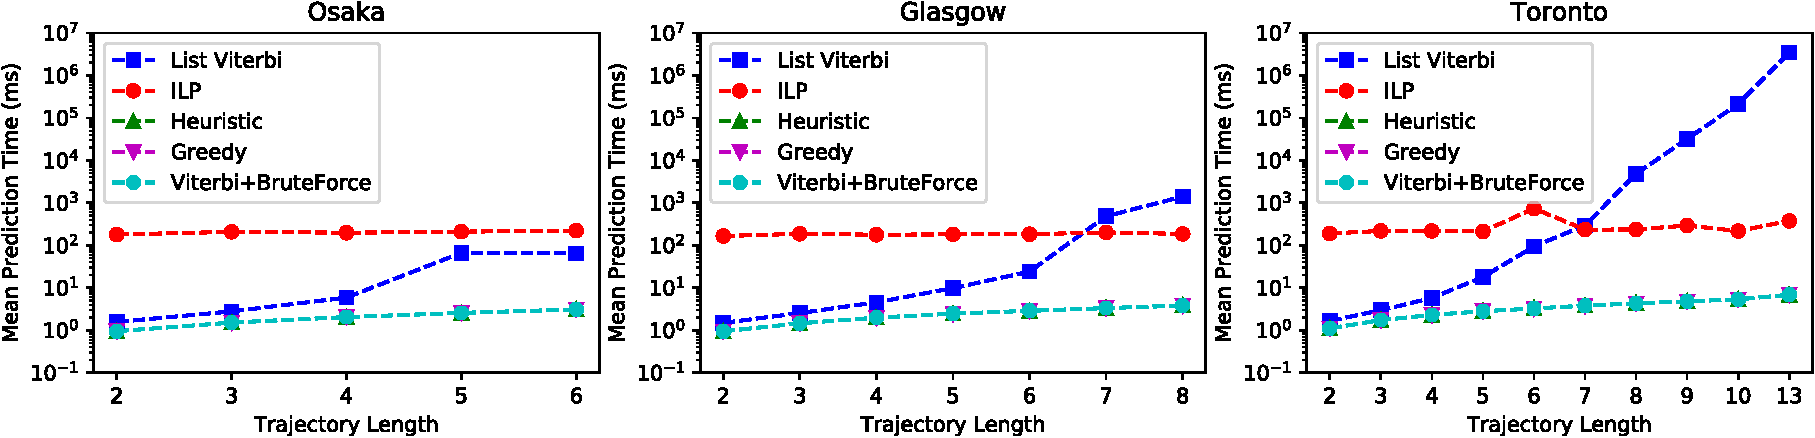
\includegraphics[width=\textwidth]{top1_inftime.pdf}
	    \captionof{figure}{Prediction time for three inference algorithms (in milliseconds)}
	    \label{fig:inftime}
	    %\captionmoveup\eqmoveup
%\end{figure*}%
%\begin{figure*}[!t]
		\quad
		\centering
		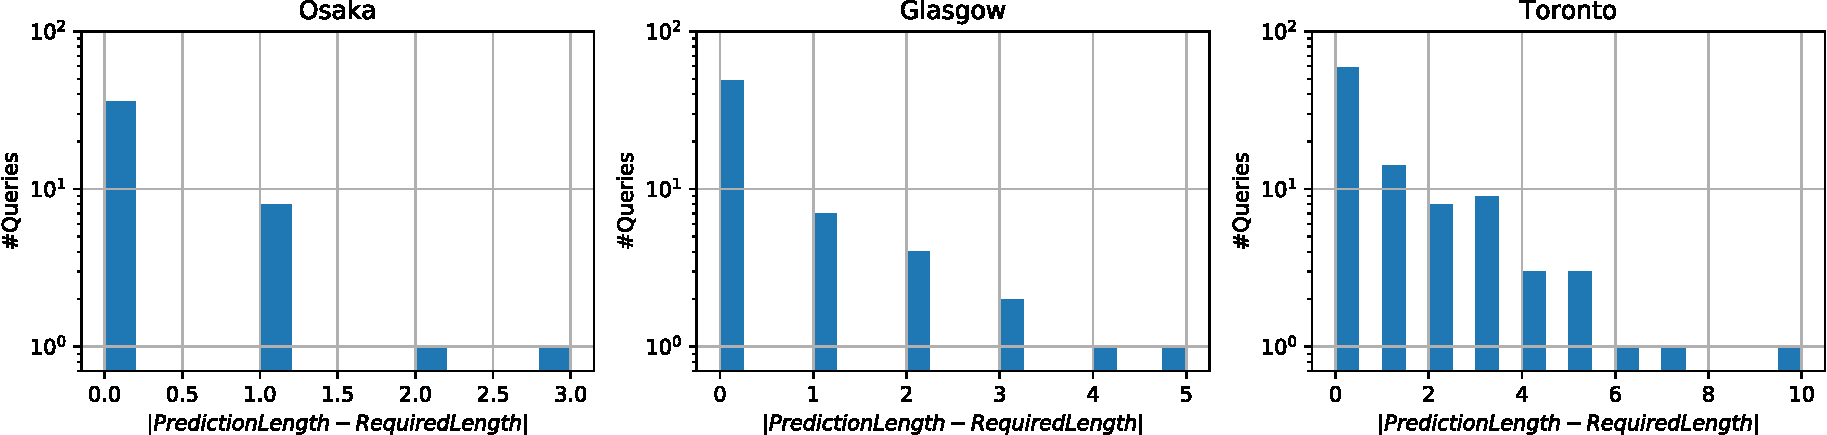
\includegraphics[width=\textwidth]{heu_lengthdiff.pdf}
	    \captionof{figure}{The difference between recommendation and required sequence length.}
	    \label{fig:length-christo}
	    %\captionmoveup\eqmoveup
%\end{figure*}%
%\begin{figure*}[!t]
		\quad
		\centering
		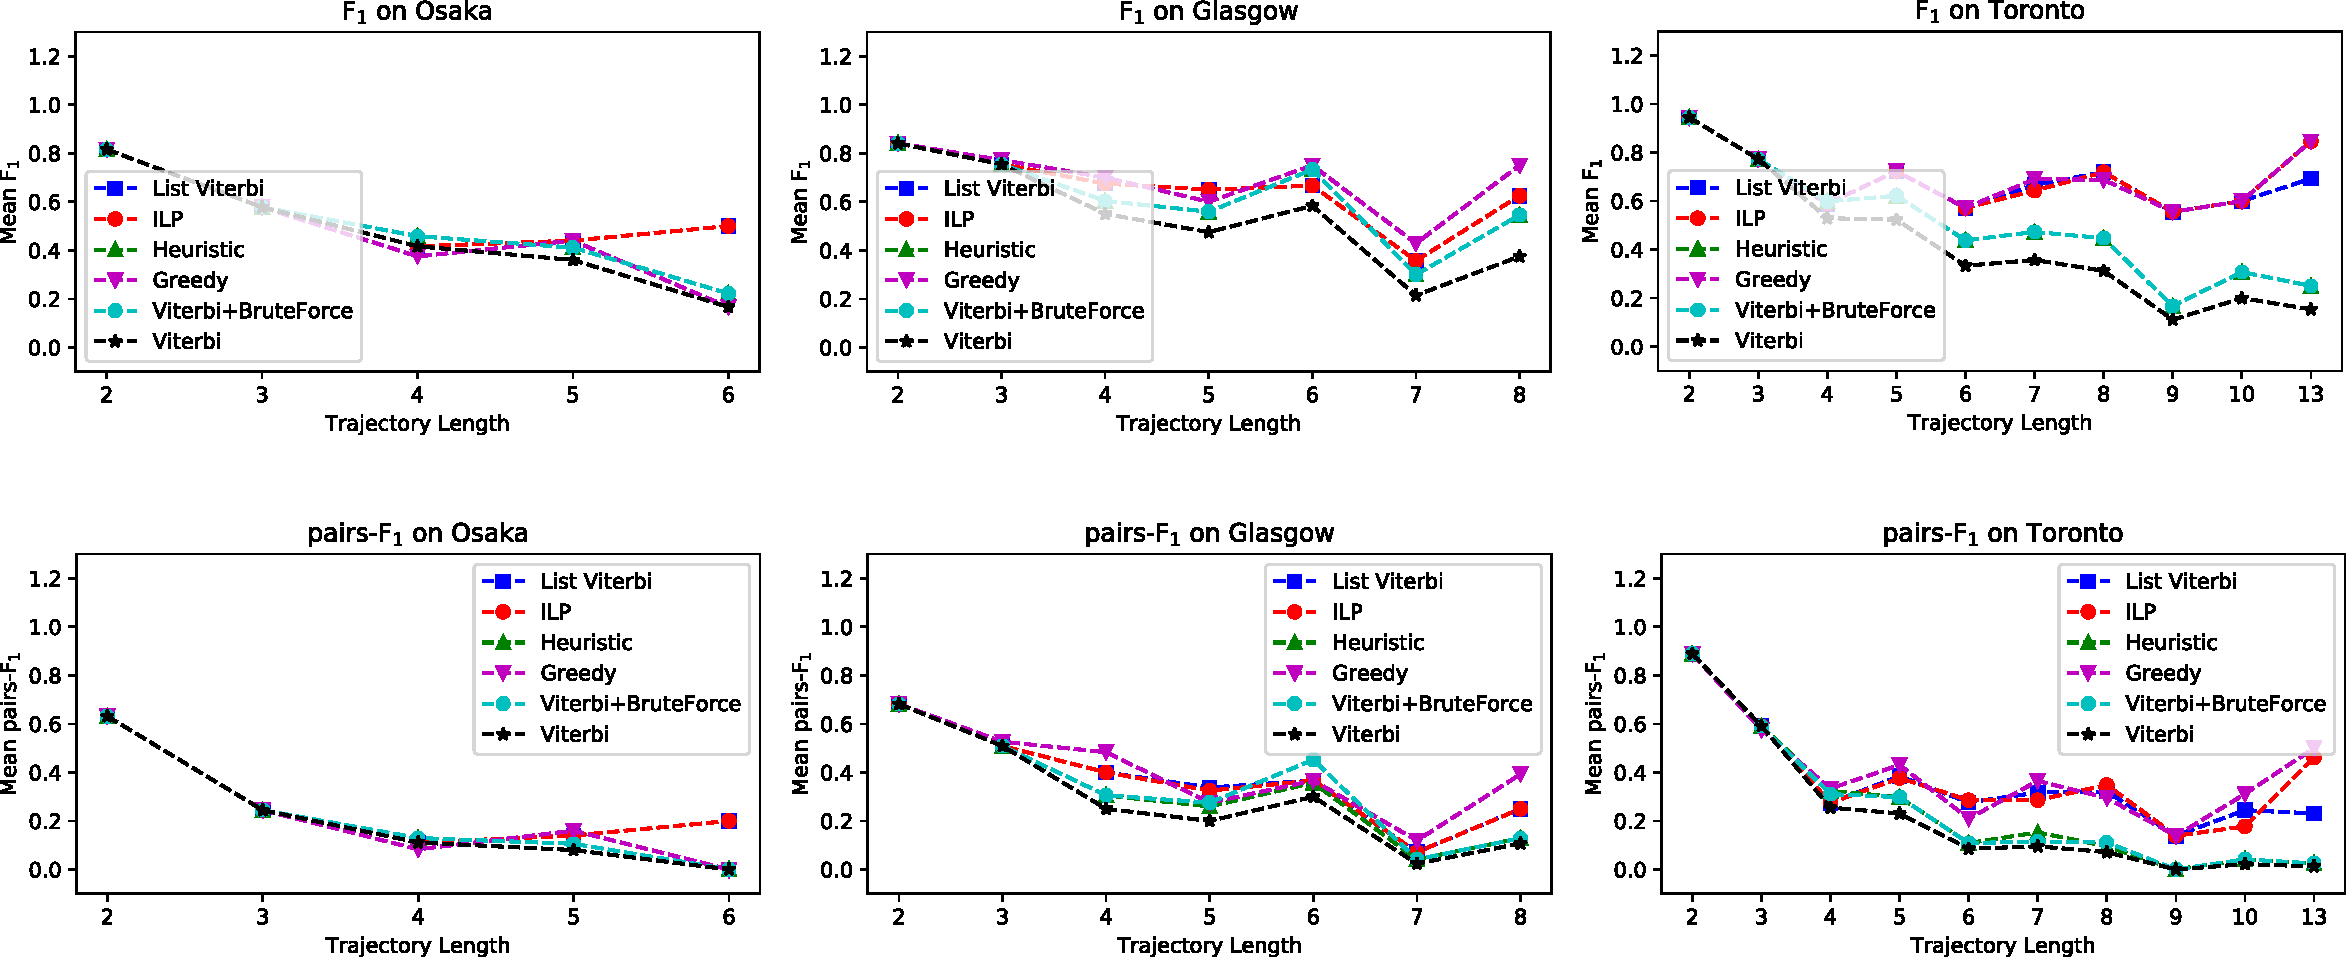
\includegraphics[width=\textwidth]{metrics.pdf}
		% 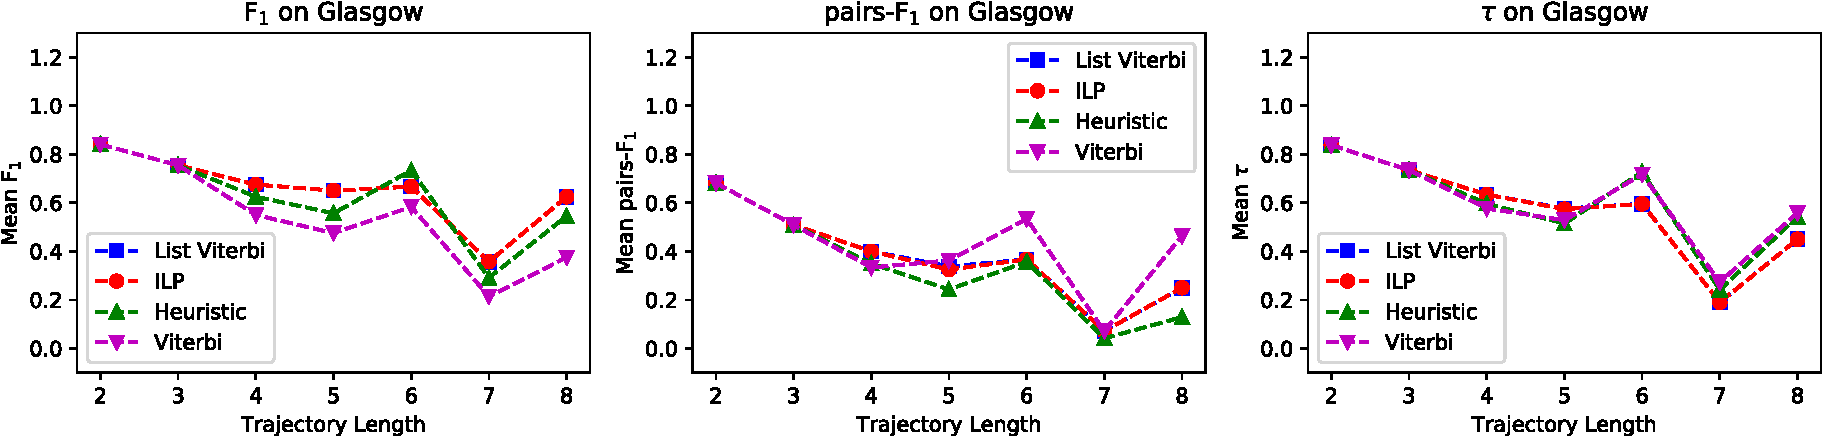
\includegraphics[width=\textwidth]{metric_d2.pdf}
		% 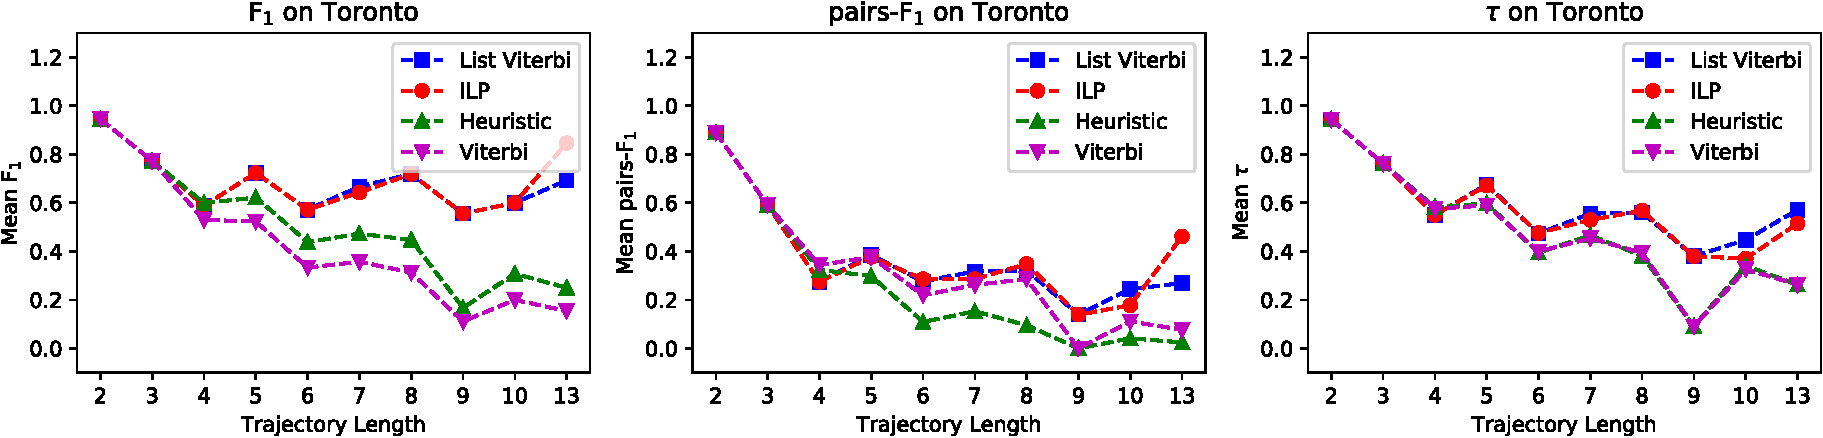
\includegraphics[width=\textwidth]{metric_d3.pdf}
	    \captionof{figure}{Accuracy versus trajectory length.}
	    \label{fig:acc-vs-length}
	    %\captionmoveup\eqmoveup
%\end{figure*}
\end{minipage}
\end{figure*}


%%%%%%%%%
\section{Discussion and Conclusion}
\label{sec:discussion}
% !TEX root=main.tex

{\color{red!75}
\begin{itemize}
	\item Learning
	\item diversity, MMR
	\item See whether any of the workshop topics might have problems that this paper applies.
\end{itemize}
}



%%%%%%%%%
\bibliographystyle{ACM-Reference-Format}
\bibliography{ref} 

\end{document}
